\documentclass[conference]{IEEEtran}
\IEEEoverridecommandlockouts
\usepackage{cite}
\usepackage{amsmath,amssymb,amsfonts}
\usepackage{algorithm}
\usepackage{algpseudocode}
\usepackage{graphicx}
\usepackage{textcomp}
\usepackage{xcolor}
\usepackage{booktabs}
\usepackage{multirow}
\usepackage{url}
\usepackage{tikz}
\usepackage{pgfplots}
\usetikzlibrary{arrows.meta,positioning,shapes.geometric,calc,fit,backgrounds,patterns}
\pgfplotsset{compat=1.17}
\usepackage{microtype}
\setlength{\textfloatsep}{6pt plus 1pt minus 1pt}
\setlength{\intextsep}{6pt plus 1pt minus 1pt}
\setlength{\dbltextfloatsep}{8pt plus 1pt minus 1pt}
\raggedbottom
\tikzset{
  stage/.style={rectangle, rounded corners=2pt, draw=black!70, fill=blue!6, minimum height=7mm, minimum width=18mm, align=center, font=\scriptsize, inner sep=2pt},
  remote/.style={rectangle, rounded corners=2pt, draw=red!70, fill=red!8, minimum height=7mm, minimum width=18mm, align=center, font=\scriptsize, inner sep=2pt},
  gate/.style={diamond, aspect=2, draw=black!70, fill=orange!12, align=center, font=\scriptsize, inner sep=1pt},
  io/.style={trapezium, trapezium left angle=70, trapezium right angle=110, draw=black!70, fill=green!8, align=center, font=\scriptsize, inner sep=2pt},
  flow/.style={-{Stealth[length=2mm]}, thick, draw=black!65},
  leak/.style={-{Stealth[length=2mm]}, thick, draw=red!75, dashed},
}
\begin{document}

\title{APEX: A Provenance-Controlled, Multi-Library\\Measurement of the Source-Attribution Ceiling\\for Stripped-Binary Functions}

\author{%
\IEEEauthorblockN{Syem Shibly Ador}
\IEEEauthorblockA{Macquarie University\\Sydney, Australia\\syemshibly.ador@mq.edu.au}
\and
\IEEEauthorblockN{Siam Shibly Antar}
\IEEEauthorblockA{McGill University\\Montreal, Canada\\siam.antar@mail.mcgill.ca}}
\maketitle

\begin{abstract}
Recovering the open-source origin of each function in a stripped binary would help
software composition analysis, vulnerability triage, and license auditing, and a
growing line of work pursues it by retrieving candidate source and verifying it,
increasingly with language models. We ask a prior question: how many functions in a
stripped binary even \emph{can} be attributed by such methods? We answer it with APEX,
a provenance-controlled, multi-library measurement. From a corpus we compile ourselves
(recorded compiler and flags), with authoritative function-to-file ground truth from
the unstripped builds, we measure at the binary level the \emph{attributability
ceiling} (CEIL): the share of functions carrying any compilation-invariant
discriminator (a rare constant, a string, or a distinctive external call) that public
code search can key on, an upper bound on what such lexical-feature retrieval can
attribute. Across thirty C
libraries the ceiling ranges from 0.0\% to 84.0\% at \texttt{-O2} (up to 72.4\% at
\texttt{-O3}, median near 32.5\%), and twenty sit below 40\%, far below what an SBOM or a
CVE check would need and independent of any verifier. Because searchability is
necessary but not sufficient, we tighten CEIL to an \emph{attributable-in-principle}
fraction, the share whose features identify a single source file; it sits 11.4 points
under the ceiling (median 21.2\%), and enlarging the reference from
fifteen to thirty libraries lowers it further (25.2\% to 22.3\% on the shared libraries),
so against all public code the gap can only widen, not close,
by an amount we do not measure. The ceiling is near-stable under static linking ($-$5.5
points) and rises about 12 points under clang, with the broad cross-library ordering
preserved. A magic-constant baseline is near-optimal where signal is constant-dominated
(F1 up to 59.8\%) and weak otherwise, and a worked-example pipeline sits at the band's
floor. The limit is on per-function attribution, not on detecting that a library is
present, which needs only one distinctive function. A second extractor on a different
disassembler and ELF parser reproduces it exactly, so the ceiling is a property of the
binaries, not the tool. We release the corpus, ground truth, extractor, and scorers.
\end{abstract}

\begin{IEEEkeywords}
binary analysis, reverse engineering, software composition analysis, software
provenance, decompilation, supply-chain security, measurement
\end{IEEEkeywords}

\section{Introduction}
A large fraction of compiled software embeds open-source components. When the
software ships stripped, the symbol table that would name each routine is gone.
Per-function attribution, mapping a binary routine to the upstream file it was compiled
from, would let an SBOM list vendored and statically linked dependencies, let a
responder decide whether a CVE applies, and substantiate license reuse.

Most prior work compares a query function to a known reference and asks whether
they match \cite{genius,gemini,safe,jtrans,trex,asm2vec}; reuse detectors report
which component is present rather than which file a routine maps to
\cite{bat,osspolice,b2sfinder,centris}; symbol-recovery methods predict a name
rather than cite a file \cite{debin,punstrip,symlm,dirty}. A newer direction
retrieves candidate source from public code and verifies it, sometimes with a
language model \cite{binaryai,llm4decompile}. All presume the target function carries enough
surviving signal to be found in the first place, a premise rarely examined.

We examine it directly with APEX (Attributability Profiling of stripped
EXecutables), a provenance-controlled measurement. Rather than proposing a tool, APEX
measures the ceiling that bounds \emph{lexical-feature} source retrieval: the fraction
of functions carrying any compilation-invariant discriminator (a rare constant, a
string, or a distinctive call name) that public code search can key on. A function
carrying none cannot be retrieved by its lexical features, however good the verifier; a
method keyed on structure instead, a learned binary-to-source embedding or call-graph
context, reads a signal the gate does not measure and falls outside CEIL. We then
tighten this upper bound to the fraction \emph{attributable in principle} and test how
the band moves across build configurations. We make the following contributions.

\begin{itemize}
\item \textbf{A provenance-controlled, multi-library corpus.} Thirty C libraries we
compile ourselves with recorded compiler and flags (one across four optimization
levels), so every binary has a known build and authoritative function-to-file ground
truth from its unstripped image.
\item \textbf{A measured attributability ceiling (CEIL).} A reproducible objdump-based
extractor gives, per binary, the fraction of functions clearing an identifiability
gate: 0.0\% to 84.0\% at \texttt{-O2} (72.4\% at \texttt{-O3}, median $\approx$32.5\%),
below 40\% for twenty of thirty.
\item \textbf{A measured band, not just a ceiling.} Tightening CEIL by intra-corpus
feature uniqueness, the \emph{attributable-in-principle} fraction sits a median 11.4
points below it (only 63\% of searchable functions are file-unique); it is an upper
bound that tightens as the reference grows (25.2\% to 22.3\% on the shared libraries as
the corpus doubles from fifteen to thirty), and is library-specific, from zero
(xxHash) to about 39 points (klib).
\item \textbf{Robustness across build axes.} The ceiling is near-stable under static
linking ($-$5.5 points) and rises about 12 points under clang's heavier inlining, with
the broad cross-library ordering preserved (Spearman $\rho=0.83$), so attributability is
build- as well as library-dependent.
\item \textbf{A diagnostic baseline.} A magic-constant lookup (near-100\% precision)
recovers most searchable signal where it is constant-dominated (xxHash, 81\% of the
ceiling) but little otherwise (zlib, 11\%); it marks where a discriminating method has room.
\item \textbf{A worked example at the floor.} A tiered retrieval-and-verification
pipeline (SRT) on a zlib binary attributes fewer than one function in ten, below both
bounds and the baseline.
\item \textbf{The ceiling is not a tool artifact.} A second extractor sharing only the
gate, on Capstone and pyelftools instead of objdump and nm, reproduces CEIL exactly on
all 2566 functions across the thirty libraries.
\end{itemize}

\section{Related Work}
\textbf{Function-level similarity.} Genius \cite{genius}, Gemini \cite{gemini},
SAFE \cite{safe}, jTrans \cite{jtrans}, Trex \cite{trex}, Asm2Vec \cite{asm2vec},
and structural diffing \cite{bindiff} compute similarity to a reference function;
they presuppose a candidate to compare against. \textbf{Reuse and license
auditing.} BAT \cite{bat}, OSSPolice \cite{osspolice}, B2SFinder \cite{b2sfinder},
BinaryAI \cite{binaryai}, and CENTRIS \cite{centris} detect components at file or package granularity.
\textbf{Symbol recovery.} DEBIN \cite{debin}, Punstrip \cite{punstrip}, SymLM
\cite{symlm}, and DIRTY \cite{dirty} predict names or types. \textbf{LLMs for
binaries.} Recent work applies language models to decompilation
\cite{llm4decompile}; our worked example uses a local code model
\cite{qwen25coder,ollama} only to adjudicate retrieval. None measures a
\emph{method-independent} ceiling on what is attributable at all: BinaryAI's recall
bound reflects one embedding model's capability, and Dramko et al.\ \cite{dramko_dimva}
measure how obfuscation degrades specific name-recovery models, not whether
discriminative signal survives compilation. CEIL is that ceiling.

\section{Measurement Method}
\subsection{Provenance-Controlled Corpus}
We compile each library ourselves and record version, compiler, exact flags, and
the SHA-256 of the stripped output. We select widely used, permissively licensed C
libraries chosen to span library types rather than to sample a population: the corpus
is thirty libraries (2566 functions), spanning
compression (zlib~1.3.1 \cite{zlib}, LZ4, miniz, heatshrink), hashing and checksums
(xxHash, sha2), cryptography (monocypher), JSON and config parsing (cJSON, yyjson,
parson, jsmn, tomlc99, inih), markdown (md4c), serialization (mpack), encoding (base64,
qrcodegen), text, string, and path utilities (utf8proc, sds, cwalk), regular expressions
(tiny-regex-c), expression evaluation (tinyexpr), networking and protocol parsing
(mongoose, http\_parser, picohttpparser), data structures (klib), logging (log.c), image
decoding (stb), tar archives (microtar), and a scripting core
(Lua's core VM), all with \texttt{gcc~13.3.0} at \texttt{-O2}, plus zlib at
\texttt{-O0/-O2/-O3/-Os}. Compiling ourselves, rather than analyzing a found binary,
is what lets us state ground truth without guessing. To probe build sensitivity, we
also recompile with \texttt{clang~18.1.3} and model static linking by recomputing CEIL
with the external-call signal (absent without a PLT) disabled.

\subsection{Ground Truth and the File-Role Criterion}
From each unstripped build we derive an authoritative address-to-function-to-file
map: per-object symbol tables give the source file, the image gives the address.
An attribution is \emph{file-role correct} if a returned candidate shares the
canonical filename of the function's true definition. Recall is over the full
eligible inventory, so a function never searched counts as a miss.

\subsection{Binary-Level Features and the Attributability Ceiling}
The quantity we measure is how many functions are searchable at all. We extract,
per function, three classes of compilation-invariant signal directly from the
compiled object with objdump and nm: rare numeric constants (immediates after
removing common and architectural values and applying a magnitude threshold,
plus a catalog of known magic constants), references into read-only data
(a proxy for string and table use), and external calls (resolved through the
PLT). A function clears the identifiability gate (Algorithm~\ref{alg:tier}) if it
carries at least one such discriminator, and the \emph{attributability ceiling}
(CEIL, Ceiling Estimation for Inferred Lineage) is the fraction of a binary's functions
that clear it. The \textsc{High}/\textsc{Medium}/\textsc{Low} tiers are inherited
from the SRT pipeline, which uses them to order search; only the \textsc{None}
versus not-\textsc{None} boundary enters CEIL. CEIL upper-bounds the recall of any
\emph{lexical-feature} retrieval method, one searching on constants, strings, or
call names as public code search does, under a perfect verifier and perfect retrieval,
because functions below it carry none of these. It does not bound a method keyed on
structure, a learned binary-to-source embedding or
call-graph context, which reads a signal the gate does not measure and can match a
feature-less function. Working from the
binary rather than from source is deliberate: macros and precomputed tables hide
constants in source that are present in the compiled image (the CRC-32 table, for
instance), so a source-level estimate undercounts.

\begin{algorithm}[t]
\caption{Identifiability gate (a function is searchable if not \textsc{None})}
\label{alg:tier}
\begin{algorithmic}[1]
\Require rare-constant count $c$, string/data-ref count $s$, external-call count $e$
\If{$c \geq 1 \wedge s \geq 1$} \Return \textsc{High}
\ElsIf{$c \geq 2 \vee s \geq 2$} \Return \textsc{High}
\ElsIf{$c \geq 1 \vee s \geq 1$} \Return \textsc{Medium}
\ElsIf{$e \geq 2$} \Return \textsc{Medium}
\ElsIf{$e \geq 1$} \Return \textsc{Low}
\Else{} \Return \textsc{None}
\EndIf
\end{algorithmic}
\end{algorithm}

\subsection{From Searchable to Attributable-in-Principle}
A discriminator enables attribution only if it is globally distinctive: a moderately
rare constant or a generic string that recurs across many files cannot pin a function
to its origin. We tighten CEIL with an intra-corpus uniqueness test: for each
searchable function we collect its identifiable features (rare-constant values, named
const-table symbols, content fingerprints of referenced read-only data, and distinctive
external callees) and index each against the source files carrying it corpus-wide. A
feature is \emph{distinctive} if every function bearing it belongs to a single source
file (by basename, so vendored copies count as one), and a function is
\emph{attributable-in-principle} if it carries at least one. A finite reference
over-counts distinctiveness, so this fraction is an \emph{upper} bound that tightens as
the reference grows: we report it against the full thirty-library corpus, and
recomputing the original fifteen libraries against a fifteen- versus thirty-library
reference shows the tightening directly, with miniz colliding with zlib on shared CRC
and deflate constants. The estimate errs on both sides, the objdump extractor missing
references it cannot resolve while the finite reference inflates it. The band geometry
is strict, CEIL $\geq$ attributable-in-principle $\geq$
realizable: retrieval returns collisions for any non-distinctive feature, so a
realizable method sits below this bound, not between it and CEIL.

\subsection{Magic-Constant Baseline}
As a floor we use a constant lookup: a function is attributed if it embeds a
globally-unique cataloged constant (CRC-32 polynomial, Adler modulus, published
xxHash primes, LZ4 frame magics). Such constants are unambiguous, so the
baseline's precision is essentially 100\%; its recall is whatever fraction of a
library's functions carry one.

\subsection{Worked Example: a Retrieval-and-Verification Pipeline}
To show what an actual pipeline achieves relative to the ceiling, we
use SRT (Fig.~\ref{fig:pipeline}): it gates functions by the same identifiability
test, builds compilation-invariant code-search queries, verifies each candidate
with a locally hosted code model, Qwen2.5-Coder-7B served by Ollama~\cite{qwen25coder,ollama}, and propagates confirmed matches
along the call graph. Read as an example, not a claim: verification is local, but the
search stage sends distinctive constants and strings to a third-party API, so the
binary is not kept private.

\begin{figure*}[t]
\centering
\resizebox{0.96\textwidth}{!}{%
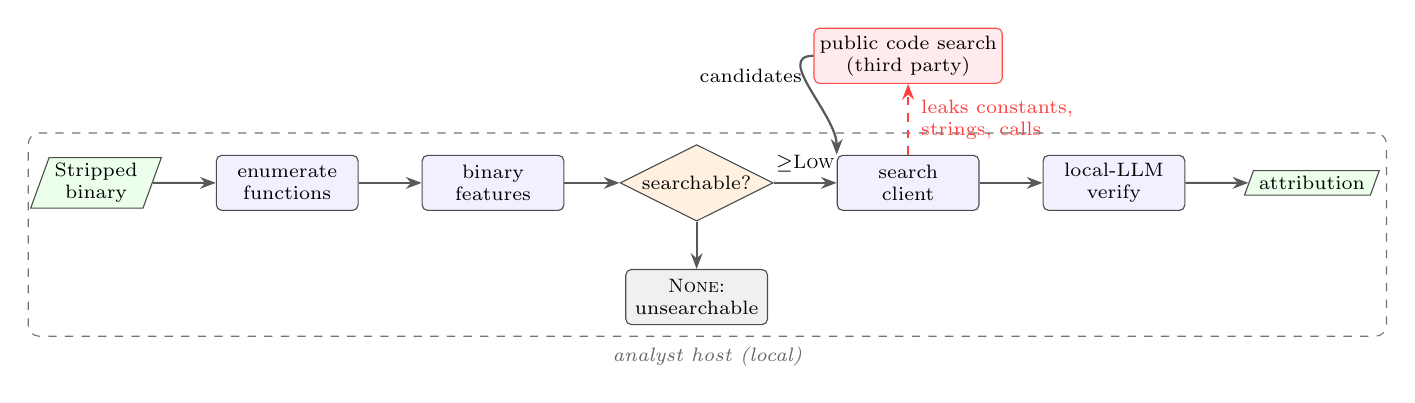
\begin{tikzpicture}[node distance=6mm and 8mm]
  \node[io] (bin) {Stripped\\binary};
  \node[stage, right=of bin] (enum) {enumerate\\functions};
  \node[stage, right=of enum] (feat) {binary\\features};
  \node[gate, right=7mm of feat] (tier) {searchable?};
  \node[stage, right=8mm of tier] (sclient) {search\\client};
  \node[stage, right=of sclient] (llm) {local-LLM\\verify};
  \node[io, right=of llm] (rep) {attribution};
  \draw[flow] (bin) -- (enum); \draw[flow] (enum) -- (feat); \draw[flow] (feat) -- (tier);
  \draw[flow] (tier) -- node[above, font=\scriptsize] {$\geq$\textsc{Low}} (sclient);
  \draw[flow] (sclient) -- (llm); \draw[flow] (llm) -- (rep);
  \node[remote, above=9mm of sclient] (gh) {public code search\\(third party)};
  \draw[leak] (sclient) -- node[right=1pt, font=\scriptsize, text=red!75, align=left] {leaks constants,\\strings, calls} (gh);
  \draw[flow] (gh.west) to[out=180,in=90] node[above left=-1pt, font=\scriptsize] {candidates} (sclient.north west);
  \node[stage, below=6mm of tier, fill=black!6] (skip) {\textsc{None}:\\unsearchable};
  \draw[flow] (tier) -- (skip);
  \begin{scope}[on background layer]
    \node[draw=black!55, dashed, rounded corners, fit=(bin)(enum)(feat)(tier)(sclient)(llm)(rep)(skip), inner sep=4pt, label={[font=\scriptsize\itshape,black!60]below:analyst host (local)}] {};
  \end{scope}
\end{tikzpicture}%
}
\caption{The worked-example pipeline. The same identifiability gate used for the
ceiling measurement decides which functions are searched. All stages are local
except code search, whose queries leak the binary's distinctive features.}
\label{fig:pipeline}
\end{figure*}

\section{Results}
\subsection{The Attributability Ceiling Across Libraries}
Fig.~\ref{fig:ceiling} shows the thirty libraries at \texttt{-O2}, and
Table~\ref{tab:ceiling} reports all thirty-three builds. The ceiling ranges from 0.0\%
(base64, whose alphabet table is mutable and so excluded by the read-only-data proxy) to
84.0\% (qrcodegen) at \texttt{-O2}, reaching 72.4\%
for zlib at \texttt{-O3}, with a median near 32.5\% and twenty of thirty below 40\%. The
pattern is interpretable: compression, hashing, checksum, and 2D-barcode code (zlib,
xxHash, qrcodegen) and table-driven text processing (utf8proc) carry distinctive
constants or large named tables and sit near the top, while parsers, serializers, and
small string, path, and archive utilities (parson, mpack, microtar, base64) carry mostly
generic control flow and ubiquitous calls and sit near the bottom. Attributability is
therefore not a property of a method but largely of the library. Because the corpus
spans library types rather than sampling a population, the median and the ``twenty below
40\%'' count describe the represented types, not functions in the wild.

\begin{figure}[t]
\centering
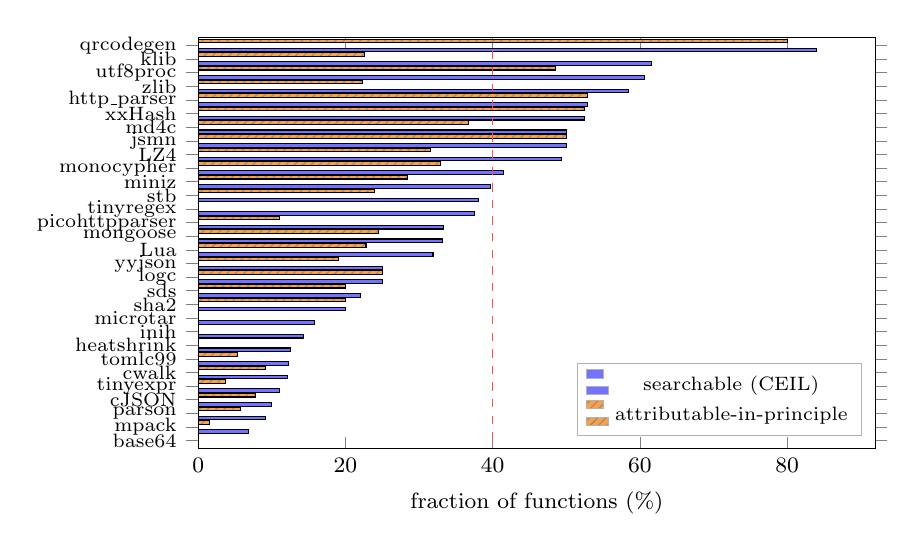
\begin{tikzpicture}
\begin{axis}[
  xbar, width=0.84\columnwidth, height=6.8cm, bar width=1.3pt,
  xmin=0, xmax=92, xlabel={\footnotesize fraction of functions (\%)},
  symbolic y coords={base64,mpack,parson,cJSON,tinyexpr,cwalk,tomlc99,heatshrink,inih,microtar,sha2,sds,logc,yyjson,Lua,mongoose,picohttpparser,tinyregex,stb,miniz,monocypher,LZ4,jsmn,md4c,xxHash,http\_parser,zlib,utf8proc,klib,qrcodegen},
  ytick=data, yticklabel style={font=\scriptsize}, xticklabel style={font=\footnotesize},
  enlarge y limits=0.02,
  legend style={font=\scriptsize, at={(0.98,0.03)}, anchor=south east, draw=black!30},
]
\addplot[fill=blue!55] coordinates {
 (0.0,base64) (6.8,mpack) (9.2,parson) (10.0,cJSON) (11.1,tinyexpr) (12.1,cwalk)
 (12.3,tomlc99) (12.5,heatshrink) (14.3,inih) (15.8,microtar) (20.0,sha2) (22.0,sds)
 (25.0,logc) (25.0,yyjson) (31.9,Lua) (33.2,mongoose) (33.3,picohttpparser) (37.5,tinyregex)
 (38.1,stb) (39.7,miniz) (41.5,monocypher) (49.4,LZ4) (50.0,jsmn) (50.0,md4c)
 (52.5,xxHash) (52.9,http\_parser) (58.5,zlib) (60.6,utf8proc) (61.6,klib) (84.0,qrcodegen)};
\addlegendentry{searchable (CEIL)}
\addplot[fill=orange!75, postaction={pattern=north east lines, pattern color=black!45}] coordinates {
 (0.0,base64) (1.6,mpack) (5.8,parson) (7.8,cJSON) (3.7,tinyexpr) (9.1,cwalk)
 (5.3,tomlc99) (0.0,heatshrink) (0.0,inih) (0.0,microtar) (20.0,sha2) (20.0,sds)
 (25.0,logc) (19.1,yyjson) (22.8,Lua) (24.5,mongoose) (11.1,picohttpparser) (0.0,tinyregex)
 (23.9,stb) (28.4,miniz) (32.9,monocypher) (31.5,LZ4) (50.0,jsmn) (36.7,md4c)
 (52.5,xxHash) (52.9,http\_parser) (22.3,zlib) (48.5,utf8proc) (22.6,klib) (80.0,qrcodegen)};
\addlegendentry{attributable-in-principle}
\draw[red!70,dashed] (axis cs:40,base64) -- (axis cs:40,qrcodegen);
\end{axis}
\end{tikzpicture}
\caption{The attributability band per library (gcc \texttt{-O2}) across the thirty-library
corpus: the searchable ceiling (CEIL) and the attributable-in-principle fraction beneath it.
The gap is the share searchable only through non-distinctive features. It is near zero for
hashing and HTTP code, whose constants and tables are unique, and among the widest for zlib and klib,
which are searchable largely through generic deflate and hash-table constants that recur
elsewhere in the corpus. The attributable line uses the thirty-library reference and is an
upper bound; an enlarged reference lowers it further. The dashed line marks 40\%.}
\label{fig:ceiling}
\end{figure}

\begin{table*}[t]
\caption{Measured binary-level attributability ceiling (CEIL) and attributable-in-principle
fraction (Attrib., judged against the full thirty-library corpus) for thirty C libraries at
gcc \texttt{-O2}, with the magic-constant baseline (recall / F1; precision $\approx$100\% by
construction, ``--'' means no cataloged constant applies). Libraries are ordered by ceiling;
the lower block is the zlib optimization sweep. All values reproducible from the released kit.}
\label{tab:ceiling}
\centering
\scriptsize
\renewcommand{\arraystretch}{0.98}
\setlength{\tabcolsep}{2.5pt}
\begin{tabular}{lrrr@{\hskip 4pt}l@{\hskip 10pt}lrrr@{\hskip 4pt}l}
\toprule
\textbf{Library} & \textbf{N} & \textbf{Ceil.} & \textbf{Attr.} & \textbf{Base. R/F1} &
\textbf{Library} & \textbf{N} & \textbf{Ceil.} & \textbf{Attr.} & \textbf{Base. R/F1} \\
\midrule
base64       & 7   & 0.0\%  & 0.0\%  & --              & mongoose       & 265 & 33.2\% & 24.5\% & -- \\
mpack        & 366 & 6.8\%  & 1.6\%  & --              & picohttpparser & 9   & 33.3\% & 11.1\% & -- \\
parson       & 120 & 9.2\%  & 5.8\%  & --              & tinyregex      & 8   & 37.5\% & 0.0\%  & -- \\
cJSON        & 90  & 10.0\% & 7.8\%  & --              & stb            & 113 & 38.1\% & 23.9\% & -- \\
tinyexpr     & 27  & 11.1\% & 3.7\%  & --              & miniz          & 141 & 39.7\% & 28.4\% & 1.4\% / 2.8\% \\
cwalk        & 33  & 12.1\% & 9.1\%  & --              & monocypher     & 82  & 41.5\% & 32.9\% & -- \\
tomlc99      & 57  & 12.3\% & 5.3\%  & --              & LZ4            & 162 & 49.4\% & 31.5\% & 11.1\% / 20.0\% \\
heatshrink   & 16  & 12.5\% & 0.0\%  & --              & jsmn           & 2   & 50.0\% & 50.0\% & -- \\
inih         & 7   & 14.3\% & 0.0\%  & --              & md4c           & 60  & 50.0\% & 36.7\% & -- \\
microtar     & 19  & 15.8\% & 0.0\%  & --              & xxHash         & 61  & 52.5\% & 52.5\% & 42.6\% / \textbf{59.8\%} \\
sha2         & 5   & 20.0\% & 20.0\% & --              & http\_parser   & 17  & 52.9\% & 52.9\% & -- \\
sds          & 50  & 22.0\% & 20.0\% & --              & zlib           & 130 & 58.5\% & 22.3\% & 6.2\% / 11.6\% \\
logc         & 8   & 25.0\% & 25.0\% & --              & utf8proc       & 33  & 60.6\% & 48.5\% & -- \\
yyjson       & 68  & 25.0\% & 19.1\% & --              & klib           & 177 & 61.6\% & 22.6\% & -- \\
Lua          & 408 & 31.9\% & 22.8\% & --              & qrcodegen      & 25  & 84.0\% & 80.0\% & -- \\
\midrule
\multicolumn{10}{l}{\textit{zlib optimization sweep:}\quad
  \texttt{-O0}: N=152, CEIL 50.0\%, base.\ 2.0\%/3.9\%\quad
  \texttt{-O3}: N=123, CEIL 72.4\%, base.\ 6.5\%/12.2\%\quad
  \texttt{-Os}: N=137, CEIL 48.9\%, base.\ 2.2\%/4.3\%} \\
\bottomrule
\end{tabular}
\end{table*}

\subsection{From Searchable to Attributable}
Fig.~\ref{fig:ceiling} overlays the attributable-in-principle fraction on CEIL (the
Attrib.\ column of Table~\ref{tab:ceiling}). Across the thirty libraries it sits 11.4
points below CEIL in the median (32.5\% versus 21.2\%); per-library gaps run from zero to
about 39 points, median 8.0, and only 63\% of searchable functions carry a globally
distinctive feature, the rest clearing the gate on constants, jump tables, or generic
data that recur across files. This is an upper bound that over-counts distinctiveness:
on the original fifteen libraries the median attributable falls from 25.2\% to 22.3\%
once the reference doubles to thirty, and zlib falls from 28.5\% to 22.3\% as miniz, an
independent deflate reimplementation, contributes the same CRC and deflate constants
from within the corpus. The direction generalizes, more reference code yields fewer
file-unique features, so against all public code the gap can only widen, not close, by
an amount we do not measure. The gap is diagnostic: zero for xxHash and http\_parser,
whose prime constants and protocol tables are unique, and among the widest for zlib and
klib, the
textbook searchable-but-not-attributable case. The bound is on \emph{lexical-feature}
retrieval; a method keyed on the call graph, as our worked example is, can attribute a
featureless function from confirmed neighbors and so sits below this line, still under
true attributability.

\subsection{The Baseline Tracks Constant-Saturation}
The constant baseline tracks constant-saturation, not the ceiling: its recall is
near-optimal where signal is unique-constant dominated and small otherwise. On xxHash,
saturated with prime magics, the matcher reaches about 81\% of the ceiling (recall
42.6\% against 52.5\%, F1 59.8\%), so a heavier pipeline has little to add. On zlib it
inverts: most searchable functions are reachable through strings, tables, and calls, so
the baseline captures roughly one-ninth of the ceiling (6.2\% against 58.5\%) and leaves
about 52 points of headroom; LZ4 falls between at roughly 22\% (11.1\% against 49.4\%).
Because the applications weight precision over recall, a precision-favoring score widens
its advantage wherever it fires, and the headroom it leaves is where a discriminating
method can operate.

\subsection{A Pipeline Operating Below the Ceiling}
We ran the SRT pipeline end to end once, on a separately obtained zlib shared object:
scored by the file-role criterion it attributes 9 of 107 eligible functions (precision
28.1\%, recall 8.4\%, F1 12.9\%). This is a worked example, not a measured comparison,
since the binary was labeled zlib~1.2.11 with its build unrecorded and is not directly
commensurable with the controlled 1.3.1 corpus. Even read loosely it sits far below the
zlib ceiling ($\approx$59\%) and loses to the constant baseline on a precision-weighted
basis, leaving most attributable headroom unused.

\subsection{Optimization Sensitivity}
On zlib the ceiling moves with optimization, from 50.0\% at \texttt{-O0} to 72.4\% at
\texttt{-O3}, with \texttt{-Os} lowest at 48.9\% (Table~\ref{tab:ceiling}): inlining
shrinks the inventory while more of the survivors carry a distinctive constant or table,
so the searchable count rises. The swing is real but narrower than the cross-library
spread, confirming attributability is build-dependent even within one library.

\subsection{Robustness across Build Axes}
Two build axes test whether the ceiling is a property of the code or of our gcc,
dynamically linked configuration. Static linking removes the PLT and the external-call
signal; disabling that signal lowers the median by only 5.5 points (32.5\% to 27.0\%),
since after filtering ubiquitous calls the searchable signal is carried by constants and
tables (a first-order model isolating the call-signal effect, not a real static binary,
which also pulls libc in). The compiler matters more: under clang the median rises about
12 points (32.5\% to 44.5\%) as heavier inlining shrinks the inventory (zlib from 130
to 81 functions) and packs signal into fewer functions, and the attributable edge rises
with it (21.2\% to 26.6\%), so the whole band shifts up rather than only its top. The
broad cross-library ordering is largely preserved (Spearman $\rho=0.83$), so
attributability is build- as well as library-dependent.

\subsection{Sensitivity of the Ceiling}
CEIL depends on three extractor choices, all swept in Fig.~\ref{fig:sens}. The
rare-constant threshold has little leverage: across a 256-fold range it moves the
median by 10.7 points (37.9\% to 27.2\%), since most functions clear the gate through a
string, table, or distinctive call rather than a borderline constant. The
call-filtering choice dominates: not filtering ubiquitous calls lifts the median from
32.5\% to 64.0\%, a 31.4-point swing, because a function whose only external call is to
\texttt{malloc} or \texttt{memcpy} then clears the gate; it is the largest lever by
about three to one, so the canonical measurement filters these calls. Third, with jump
tables already discounted (an indirect-jump target is not counted as data), restricting
the rest to named const tables lowers the canonical median by 7.5 points, the share
reachable only through anonymous read-only tables the extractor does not name.

\begin{figure}[t]
\centering
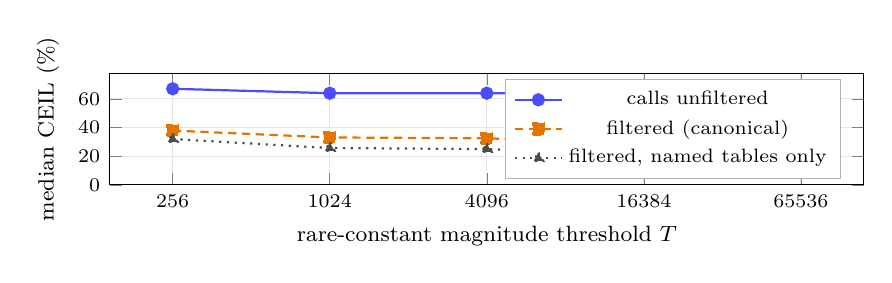
\begin{tikzpicture}
\begin{axis}[
  width=0.92\columnwidth, height=3.0cm,
  xmode=log, log basis x=2,
  xtick={256,1024,4096,16384,65536}, xticklabels={256,1024,4096,16384,65536},
  xlabel={\footnotesize rare-constant magnitude threshold $T$},
  ylabel={\footnotesize median CEIL (\%)},
  ymin=0, ymax=78,
  tick label style={font=\scriptsize}, label style={font=\footnotesize},
  legend style={font=\scriptsize, at={(0.97,0.5)}, anchor=east, draw=black!30},
  grid=major, grid style={black!10},
]
\addplot[mark=*, thick, solid, blue!70] coordinates {(256,67.1)(1024,64.0)(4096,64.0)(16384,64.0)(65536,62.8)};
\addlegendentry{calls unfiltered}
\addplot[mark=square*, thick, densely dashed, orange!90!black] coordinates {(256,37.9)(1024,33.1)(4096,32.5)(16384,28.4)(65536,27.2)};
\addlegendentry{filtered (canonical)}
\addplot[mark=triangle*, thick, dotted, black!70] coordinates {(256,32.0)(1024,25.7)(4096,25.0)(16384,20.3)(65536,20.3)};
\addlegendentry{filtered, named tables only}
\end{axis}
\end{tikzpicture}
\caption{Sensitivity of the median ceiling across the thirty libraries. The
rare-constant threshold (x-axis, log scale) moves the median by 10.7 points, and
restricting data references to named const tables by 7.5; filtering ubiquitous libc
and runtime calls moves it by 31.4. The canonical setting filters calls and
counts both named and anonymous (jump-table-discounted) tables.}
\label{fig:sens}
\end{figure}

\subsection{Component Detection versus Per-Function Attribution}
Per-function attribution and library-presence detection are different questions, and
the ceiling answers the first. Detecting presence needs only one attributable function;
attributing every function needs them all. A library with $N$
functions, $A$ of them file-attributable, that contributes $k$ functions to a binary
is detectable in principle with probability $1-\binom{N-A}{k}/\binom{N}{k}$, an
upper bound for the same reason the ceiling bounds attribution and treating the draw as
uniform (real dead-code elimination is reachability-driven). At $k=1$ this equals the
per-function attributable fraction; once the whole library links it is one whenever
$A\geq1$. Fig.~\ref{fig:detect} plots it. The median per-function attributable fraction
is 21.2\%, but ten linked functions include a distinctive one with median probability
92.8\%, and 25 of the 30 fully linked libraries carry at least one. Five small libraries
(base64, heatshrink, inih, microtar, and tinyregex) carry no file-attributable function
at all, so they are undetectable in principle by this signal even when fully linked. The
function behind CVE-2022-37434, a heap over-read in zlib's \texttt{inflate}, stays
file-attributable even with miniz, an independent deflate reimplementation, in the
corpus, so the affected component is locatable; pinning the specific vulnerable version
is a strictly harder bar the file-level ceiling does not address. Per-function
attribution is fundamentally limited; detecting a present component in principle, the
target of tools such as OSSPolice and CENTRIS, is not, and the two diverge because
presence needs a single distinctive function while attribution needs the whole set.

\begin{figure}[t]
\centering
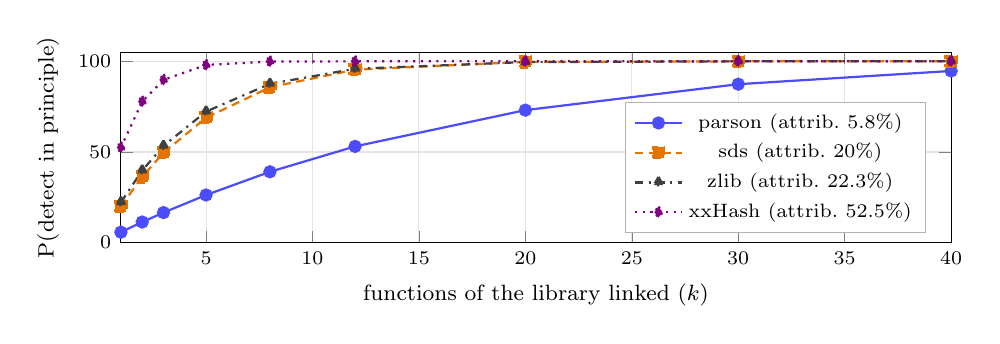
\begin{tikzpicture}
\begin{axis}[
  width=\columnwidth, height=4.0cm,
  xlabel={functions of the library linked ($k$)},
  ylabel={P(detect in principle)}, ylabel style={font=\footnotesize},
  xlabel style={font=\footnotesize},
  xmin=1, xmax=40, ymin=0, ymax=105,
  tick label style={font=\scriptsize},
  legend style={font=\scriptsize, at={(0.97,0.05)}, anchor=south east, draw=black!30},
  grid=major, grid style={black!10},
]
\addplot[mark=*, thick, solid, blue!70] coordinates {(1,5.8)(2,11.4)(3,16.6)(5,26.3)(8,39.1)(12,53.1)(20,73.1)(30,87.4)(40,94.7)};
\addlegendentry{parson (attrib.\ 5.8\%)}
\addplot[mark=square*, thick, densely dashed, orange!90!black] coordinates {(1,20.0)(2,36.3)(3,49.6)(5,68.9)(8,85.7)(12,95.4)(20,99.7)(30,100)(40,100)};
\addlegendentry{sds (attrib.\ 20\%)}
\addplot[mark=triangle*, thick, dashdotted, black!75] coordinates {(1,22.3)(2,39.8)(3,53.4)(5,72.3)(8,87.6)(12,95.9)(20,99.6)(30,100)(40,100)};
\addlegendentry{zlib (attrib.\ 22.3\%)}
\addplot[mark=diamond*, thick, dotted, violet] coordinates {(1,52.5)(2,77.8)(3,89.8)(5,98.0)(8,99.9)(12,100)(20,100)(30,100)(40,100)};
\addlegendentry{xxHash (attrib.\ 52.5\%)}
\end{axis}
\end{tikzpicture}
\caption{Probability that a present library is detectable in principle as a function
of how many of its functions the binary links, for four libraries spanning the ceiling
range. The legend gives each library's attributable fraction, where its curve begins
at $k=1$; detection saturates well before a library is fully linked even when that
fraction is low, because presence needs only one distinctive function.}
\label{fig:detect}
\end{figure}

\subsection{Independent-Extractor Validation}
\label{sec:validation}
To test whether the ceiling reflects the binaries or how we read objdump's output, we
re-derive CEIL with a second pipeline sharing only the gate: it disassembles with
Capstone~\cite{capstone} and reads symbols and relocations with
pyelftools~\cite{pyelftools}, replacing objdump and nm, while the rare-constant test,
magic catalog, libc filter, and jump-table discount are imported unchanged. The two
agree on every one of the 2566 functions across all thirty libraries (mean absolute
difference 0.0 points), so CEIL is a property of the compiled code under a fixed gate,
not of the objdump text interface. The released kit runs both.

\section{Discussion}
\textbf{Attributability is bounded and library-dependent.} For twenty of thirty
libraries the ceiling sits below 40\%, and below 15\% for the smallest parsers and
utilities. No verifier can attribute a function that carries no lexical signal, so
these ceilings cap every lexical-feature method; one keyed on structure or call-graph
context, as our worked example is, reads a different signal and is the exception.
Per-function attribution is thus most effective on constant-rich code and weak on the
parsing and glue code that dominates many binaries.

\textbf{Searchable is not attributable.} Over a third of searchable functions carry only
non-distinctive signal, and for zlib the searchable fraction is more than twice the
attributable one; enlarging the reference only widens the gap. Reported as a single
number, searchability overstates what attribution can achieve, and the gap names where
a method is retrieval-limited rather than verification-limited.

\textbf{The baseline is competitive where signal is constant-dominated.} The ceiling
rests on constants: removing the rare-constant signal drops the median by 12.3 points,
against 1.2 for data references and 0 for distinctive calls. A constant lookup is
therefore near-optimal where constants dominate, and a heavier pipeline, which our
worked example did not beat, has room only where they do not.

\section{Limitations and Future Work}
Our extractor approximates a decompiler's feature set from objdump and nm, a
conservative proxy, and the gate admits any single discriminator, so the ceilings
carry two-sided error quantified by the sensitivity sweep (Fig.~\ref{fig:sens}). Four
directions remain. \emph{Deeper validation}: the Capstone/pyelftools extractor already
reproduces CEIL exactly, so a decompiler-based extractor (Ghidra~\cite{ghidra} or IDA)
would test the feature set itself, and an oracle test of whether any \textsc{None}-tier
function is attributable from structure would confirm the gate is a true floor.
\emph{The realizable rung}: a controlled
retrieval-and-verification experiment over a fixed candidate set of true source plus
distractors, with an oracle variant, would locate where a strong method lands within the
band and separate retrieval- from verification-limited loss. \emph{Breadth}: the corpus
is thirty x86-64 C libraries spanning many types but still weighted toward small ones,
so other instruction sets (aarch64) and formats (PE) need an extractor port, and a larger
stratified corpus with real stripped artifacts (sqlite, openssl, busybox, firmware) would
turn this type-spanning distribution into a population-level estimate. \emph{Version
attributability}: because the distinctiveness test collapses by basename it answers which
file, whereas CVE triage needs which version, so the share of file-attributable functions
carrying release-pinning features is the harder quantity the application requires. The
released harness supports each; none changes the central result that most parsing and
glue code is not attributable by content.

\section{Conclusion}
With APEX we measured how attributable the functions of a stripped binary are, across
thirty C libraries with controlled provenance and ground truth. The searchable ceiling
is strongly library-dependent (0.0\% to 84.0\% at \texttt{-O2}, 72.4\% at \texttt{-O3},
median $\approx$32.5\%) and below 40\% for most; intra-corpus uniqueness tightens it to an
attributable-in-principle bound 11.4 points lower, and lower still as the reference grows
from fifteen to thirty libraries. The band is stable under static linking and shifts
upward under clang, and a worked-example pipeline sits at its floor. Across the types we
sample, lexical-feature attribution is often fundamentally limited, and that limit, not
verifier quality, should frame future work.

\section*{Reproducibility and Artifacts}
We release the APEX kit: provenance-pinned gcc and clang build scripts, the
ground-truth extractor, the ceiling, uniqueness, baseline, sensitivity, decomposition,
and component-detection analyzers, the independent Capstone/pyelftools cross-check, and
the file-role scorer. Every number in Figs.~\ref{fig:ceiling}, \ref{fig:sens},
and~\ref{fig:detect} and Table~\ref{tab:ceiling} reproduces from the released tags, at
\url{https://github.com/REPLACE-ME/apex} (Zenodo DOI~\texttt{REPLACE-ME}).
% TODO(author): replace the repository URL and the Zenodo DOI before camera-ready.

\bibliographystyle{IEEEtran}
\bibliography{references}
\end{document}